\section{Results}
\label{sec:results}

\subsection{Belief Space Is Low-Dimensional}

\tabref{tab:variance} summarizes the number of principal components required to reach four variance thresholds across our three PCA methods and the random baseline.

\begin{table}[t]
\centering
\caption{Number of principal components needed to explain a given fraction of total variance. Persona response PCA requires 40\% fewer components than the random baseline at the 90\% threshold. Conditional influence PCA is even more compressed: 25 components suffice for 90\%.}
\label{tab:variance}
\vspace{4pt}
\resizebox{\textwidth}{!}{%
\begin{tabular}{@{}lcccc@{}}
\toprule
Threshold & Semantic Embedding (9,993) & Persona Response (300) & Conditional Influence (50$\times$100) & Random Baseline \\
\midrule
50\%  & 46  & {\bf 9}   & {\bf 5}   & 55  \\
80\%  & 200 & {\bf 56}  & {\bf 16}  & 117 \\
90\%  & 380 & {\bf 93}  & {\bf 25}  & 154 \\
95\%  & 501 & {\bf 127} & {\bf 32}  & --- \\
\bottomrule
\end{tabular}%
}
\end{table}

The persona response PCA is strikingly compact. Only 9 components capture 50\% of variance, compared to 55 for random data---a 6$\times$ compression. At the 90\% threshold, 93 components suffice versus 154 for random, a 40\% reduction. The conditional influence structure is even sparser: just 5 components explain 50\% of belief-to-belief influence, and 25 explain 90\%.

The Kaiser criterion (eigenvalue $> 1$) identifies 60 significant components in the response PCA, consistent with the 56 components needed for 80\% variance. In semantic embedding space, 251 components pass the Kaiser threshold, reflecting the high topical diversity of the belief corpus.

\subsection{The Progressive--Conservative Axis Dominates}

The first principal component of the persona response PCA explains 28.6\% of total variance---95$\times$ more than the $\sim$0.3\% expected for a single component under the random baseline. This component maps cleanly to a progressive--conservative ideological axis (\tabref{tab:pc1}).

\begin{table}[t]
\centering
\caption{Top beliefs loading on PC1 of the persona response PCA (28.6\% of variance). Positive loadings correspond to progressive/liberal positions; negative loadings correspond to conservative/traditional positions.}
\label{tab:pc1}
\vspace{4pt}
\resizebox{\textwidth}{!}{%
\begin{tabular}{@{}lr@{}}
\toprule
Belief statement & Loading \\
\midrule
\multicolumn{2}{@{}l}{\em Positive (progressive)} \\
\cmidrule(lr){1-2}
``The criminal justice system ought to focus more on restorative justice'' & $+0.100$ \\
``Harm reduction programs like needle exchanges are essential'' & $+0.099$ \\
``National boundaries are socially constructed limitations'' & $+0.098$ \\
\midrule
\multicolumn{2}{@{}l}{\em Negative (conservative)} \\
\cmidrule(lr){1-2}
``Criminals must first be held accountable through punishment'' & $-0.097$ \\
``Wealth inequality reflects differences in individual effort and talent'' & $-0.097$ \\
``Police officers should be given broad authority to use force'' & $-0.097$ \\
\bottomrule
\end{tabular}%
}
\end{table}

\subsection{Higher Components Capture Distinct Dimensions}

Beyond the ideological axis, subsequent components capture interpretable dimensions (\figref{fig:loadings}):

\begin{itemize}[leftmargin=*,itemsep=0pt,topsep=0pt]
    \item {\bf PC2} (5.8\%): Institutional trust vs.\ skepticism. High scorers express concerns about automation, neocolonialism, and institutional overreach; low scorers express satisfaction with democratic processes and market mechanisms.
    \item {\bf PC3} (4.6\%): Communitarianism vs.\ individualism. High scorers emphasize community duty, mutual obligation, and tradition; low scorers favor tech-forward individualism.
    \item {\bf PC4} (3.6\%): Spiritual vs.\ secular worldview. High scorers endorse spiritual enlightenment and absolute moral truths; low scorers prioritize secular, pragmatic concerns.
    \item {\bf PC5} (2.2\%): Gender equality attitudes. This component separates beliefs about women in leadership and gender barriers.
\end{itemize}

Together, the top five components explain 44.8\% of total variance. This five-dimensional model aligns with known findings from the World Values Survey~\cite{inglehart2005modernization}, which identifies traditional--secular and survival--self-expression axes, while adding finer-grained dimensions that emerge from our larger belief corpus.

\begin{figure}[t]
\centering
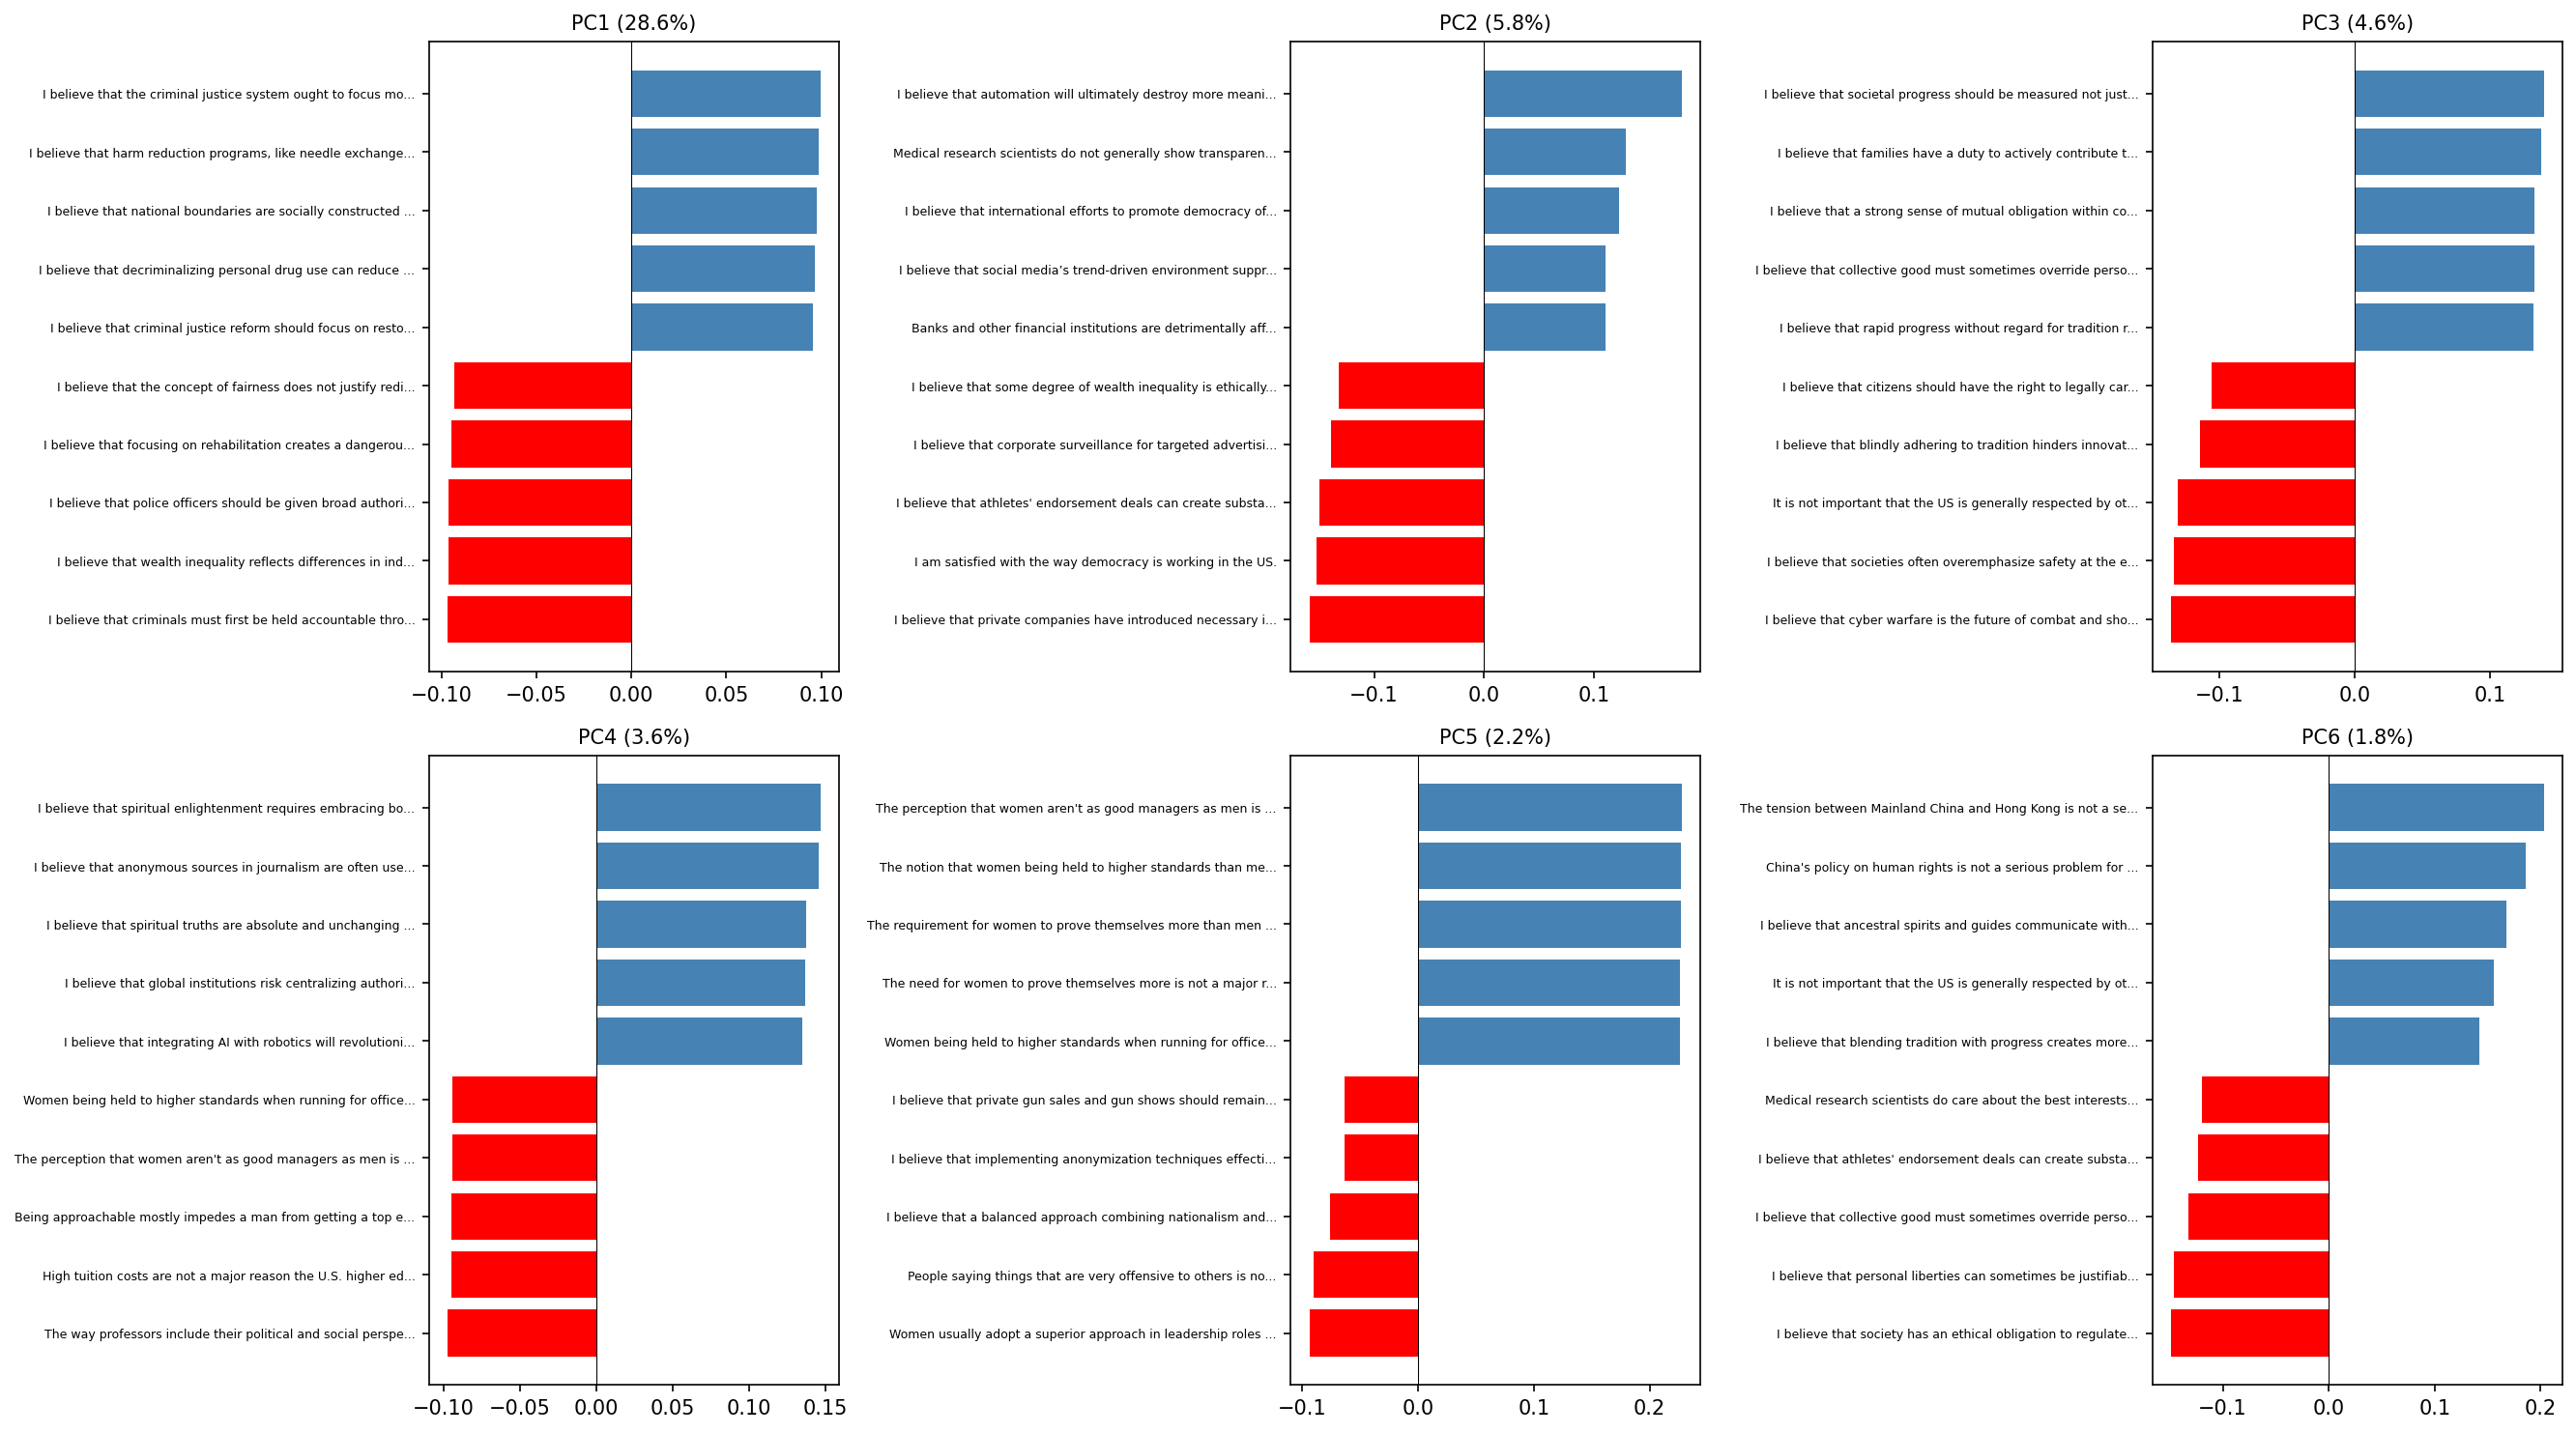
\includegraphics[width=0.95\linewidth]{../results/plots/response_pca_loadings.png}
\caption{Top belief loadings on the first six principal components of the persona response PCA. PC1 captures a progressive--conservative axis; subsequent components capture institutional trust, individualism, spirituality, and gender attitudes.}
\label{fig:loadings}
\end{figure}

\subsection{Semantic vs.\ Attitudinal Dimensionality}

\begin{figure}[t]
\centering
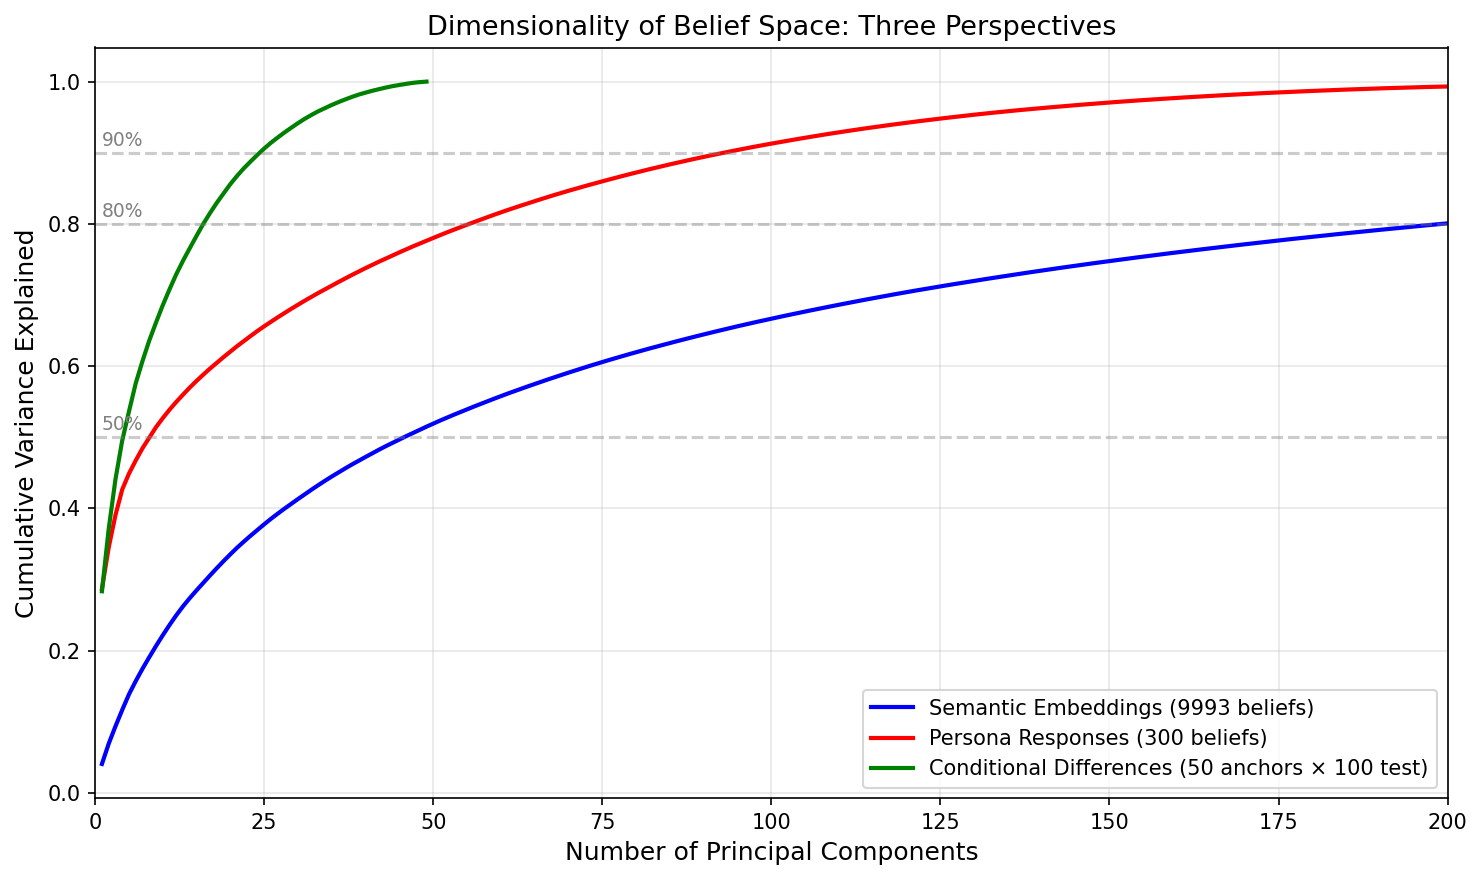
\includegraphics[width=0.95\linewidth]{../results/plots/comparison_cumvar.png}
\caption{Cumulative variance explained by the three PCA methods. Semantic embedding PCA (blue) is the most diffuse, reflecting high topical diversity. Persona response PCA (orange) is substantially more compact, indicating that attitudinal covariance is far simpler than topical diversity. Conditional influence PCA (green) is the most compressed, showing that the causal structure of beliefs is even lower-dimensional.}
\label{fig:comparison}
\end{figure}

\figref{fig:comparison} reveals a striking gap between semantic and attitudinal dimensionality. Semantic embedding PCA requires 380 components for 90\% variance, while persona response PCA needs only 93---a 4$\times$ difference. This confirms that semantically dissimilar beliefs (\eg gun rights and economic individualism) can covary strongly, and that the latent structure governing {\em who holds which beliefs} is far simpler than the topical landscape of {\em what beliefs exist}.

\subsection{Conditional Influence Analysis}

\begin{figure}[t]
\centering
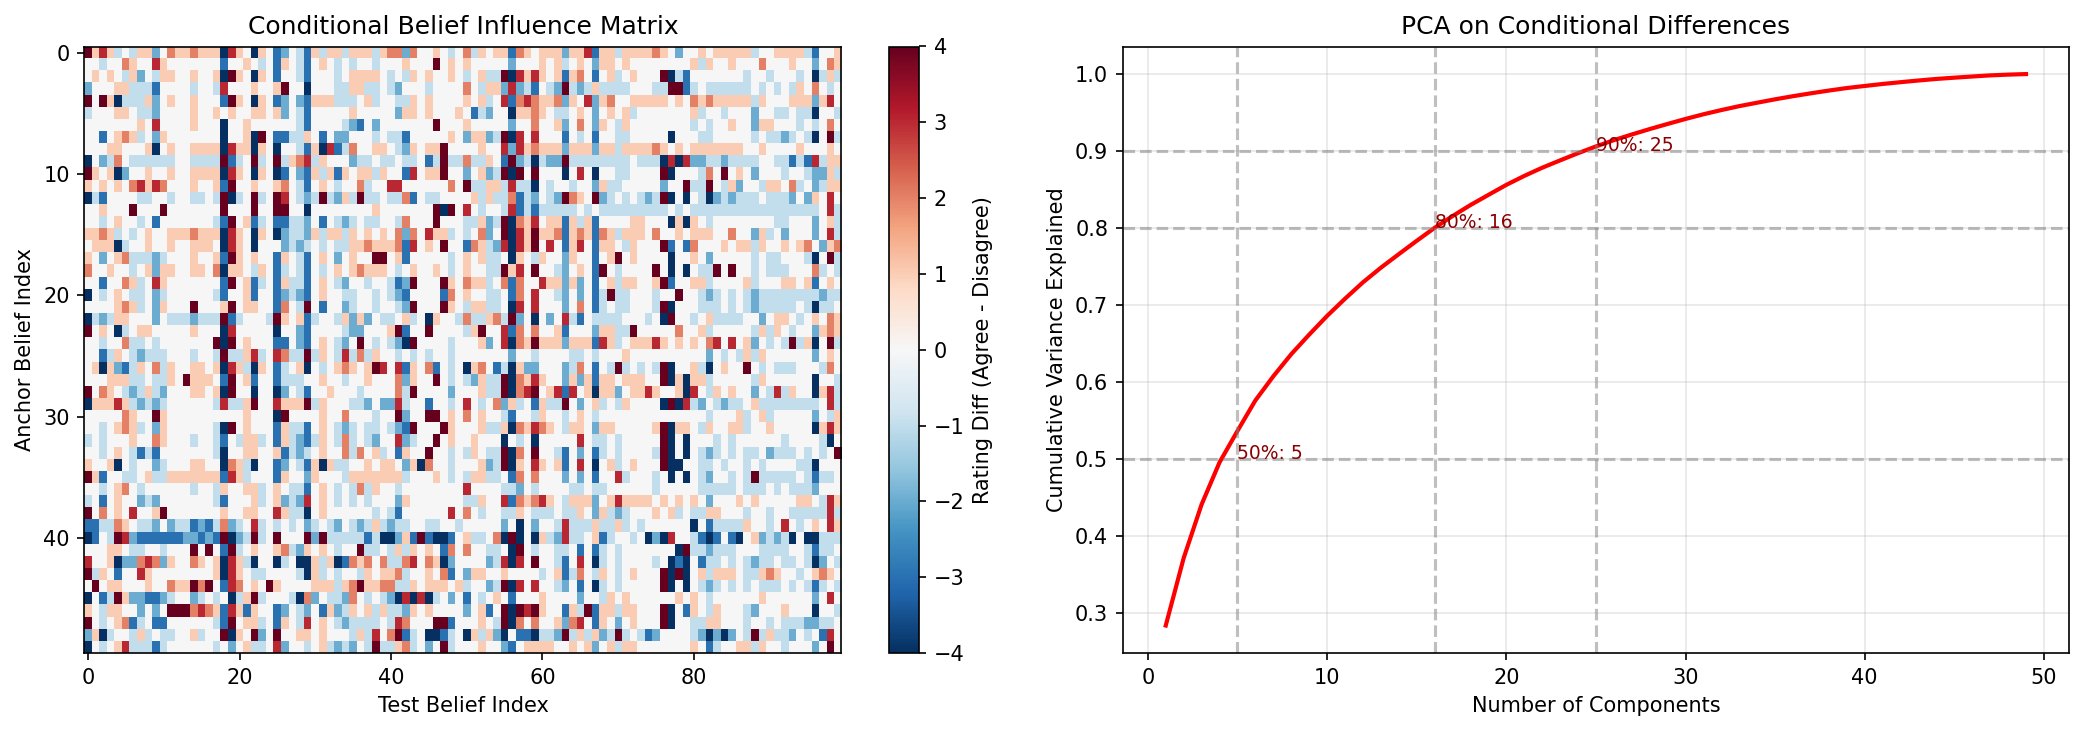
\includegraphics[width=0.95\linewidth]{../results/plots/conditional_belief_analysis.png}
\caption{Conditional belief influence analysis. The matrix (left) shows how agreement or disagreement with anchor beliefs (rows) shifts predicted ratings of test beliefs (columns). PCA on this matrix (right) reveals that 25 dimensions capture 90\% of the influence structure.}
\label{fig:conditional}
\end{figure}

The conditional influence experiment (\figref{fig:conditional}) measures how much knowing someone's stance on one belief changes our prediction of their other stances. The highest-impact anchor beliefs are:

\begin{enumerate}[leftmargin=*,itemsep=0pt,topsep=0pt]
    \item ``Economic success is the only legitimate measure of merit'' (impact: 2.07)
    \item ``Animal testing for cosmetics should be banned globally'' (impact: 1.48)
    \item ``Countries should enforce absolute border closures'' (impact: 1.47)
\end{enumerate}

The most {\em sensitive} beliefs---those whose predicted ratings shift most depending on which anchor is held---include ``Attempts to ban high-capacity magazines infringe on rights'' (sensitivity: 2.96) and ``The state's primary role should be limited to protecting from force/fraud'' (sensitivity: 2.80). These high-sensitivity beliefs are the most diagnostic of someone's overall worldview.

\subsection{Response Distribution}

The rating distribution across all persona--belief pairs is right-skewed (mean 3.97, std 1.23), with the modal response being 5 (Strongly Agree; 40,398 of 90,000 ratings). This skew reflects that many beliefs were phrased as positive or aspirational statements. Despite this compression, strong covariance structure persists, suggesting our dimensionality estimates may be conservative---more balanced phrasing could reveal even richer structure.

\begin{figure}[t]
\centering
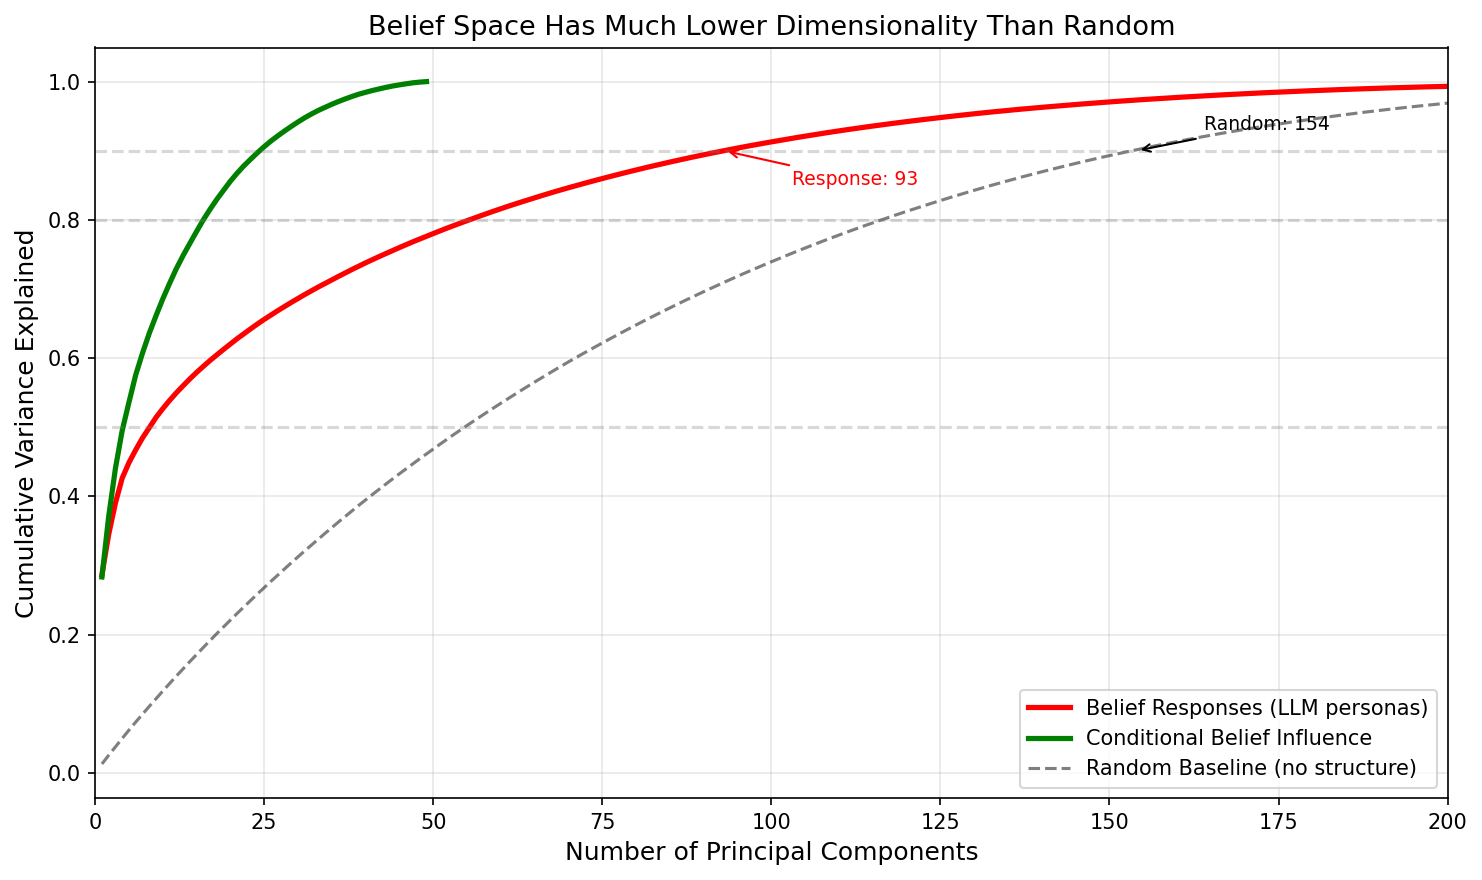
\includegraphics[width=0.95\linewidth]{../results/plots/response_vs_random.png}
\caption{Cumulative variance explained for persona response PCA (solid) vs.\ random baseline (dashed). The belief data concentrates variance far more rapidly than random, with PC1 alone explaining 28.6\% vs.\ $\sim$0.3\% for random.}
\label{fig:vsrandom}
\end{figure}
